\begin{document}
%=================================================================
%                           Start Document
%=================================================================
\section{System Design}
\lhead{System Design} % section header

\subsection{Functional Electrical Stimulation}

\subsubsection{Electrode configuration}
There are two main configuration for electrical activation of neuromuscular tissue. There is bipolar stimulation in which each stimulation cite has an active electrode placed near the peripheral nerve and a reference electrode close by. The other configuration is monopolar where the return electrode is placed in a remote area near less excitable tissue \cite{peckham_functional_2005}. 
This approach reduces the number of leads and electrodes required, however for multichannel systems bipolar stimulation may allow greater selectivity of activation because each electrode par creates a more localized electric field \cite{grandjean_recruitment_1986}. 

\subsubsection{Stimulation waveform}
Stimulus waveforms are generally monophasic or biphasic. Monophasic waveforms consist of a single phase of electrical current delivered in one polarity, while Biphasic waveforms consist of a cathodic phase followed by an anodic phase. This mitigates the buildup of charge at the electrode-tissue interface by ensuring that the net charge delivered over time is zero, effectively reducing the risk of tissue damage as compared to monophasic waveforms \cite{peckham_functional_2005}. Additionally the biphasic rectangular stimulation is the most commonly used, as it offers the best force-amplitude ratio
\cite{lynch_functional_2008}. For these reasons the balanced biphasic rectangular waveform was chosen for the stimulation protocol.
 \begin{figure} [H]
     \centering
     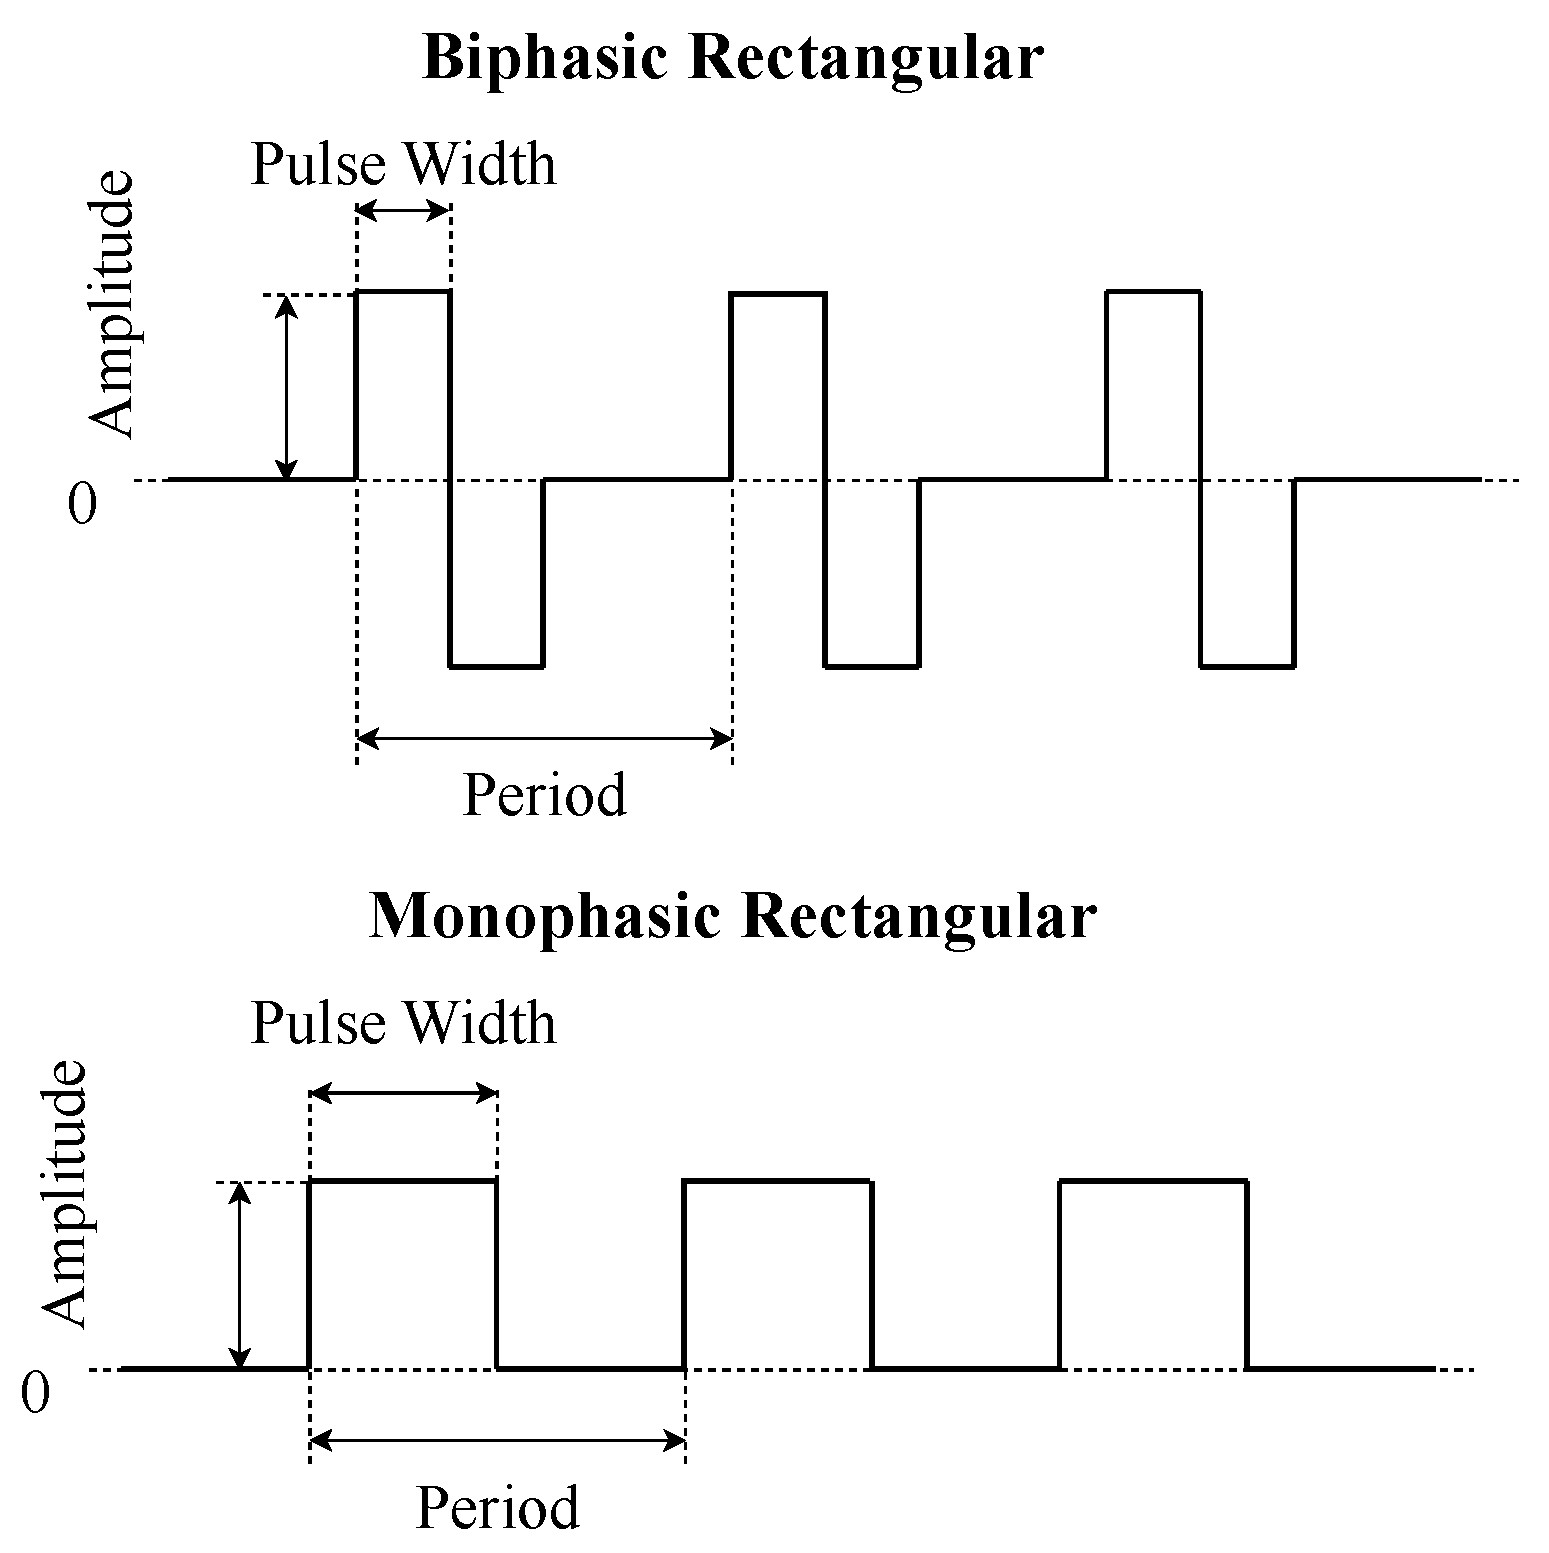
\includegraphics[width=0.6\linewidth]{images/twowaveform.jpg}
     \caption{Caption}
     \label{fig:enter-label}
 \end{figure}

\subsubsection{Stimulation frequency}
The stimulation frequency affects the strength of the contraction and its quality. A higher frequency will lead to the force produced by each subsequent pulse being added so that the mean force of the contraction is greater than that produced by a single twitch. Further increase in frequency results in sustained contraction which produces a smooth movement instead of individual twitches. The minimum frequency required to induce fairly consisten contraction is between 16 and 20 Hz \cite{marquez-chin_functional_2020}. A smoother contraction is also more comfortable for the patient. However one should not use a higher frequency than necessary since it has been observed that fatigue accumulated in a muscle is related to the number of pulses received. Therefore when choosing the stimulation frequency the aim was to choose the lowest frequency that still produced sustained contractions. In a clinical environment, the typical range of frequencies is around 20-50Hz, and during literature review it was observed that the majority of teams using FES on gait are using a stimulation frequency around 40Hz \cite{aout_effects_2023}. Therefore the same 40Hz stimulation frequency was chosen for this project.

\begin{}


%=================================================================
%                           End Document
%=================================================================
\end{document}